\section{Comparison of 3 Computer Vision Models}
\label{sxn:cv}

\paragraph{Empirical Metrics vs Test Accuracies for VGG}

\begin{figure}[t]
    \centering
    \subfigure[ Frobenius Norm ]{
        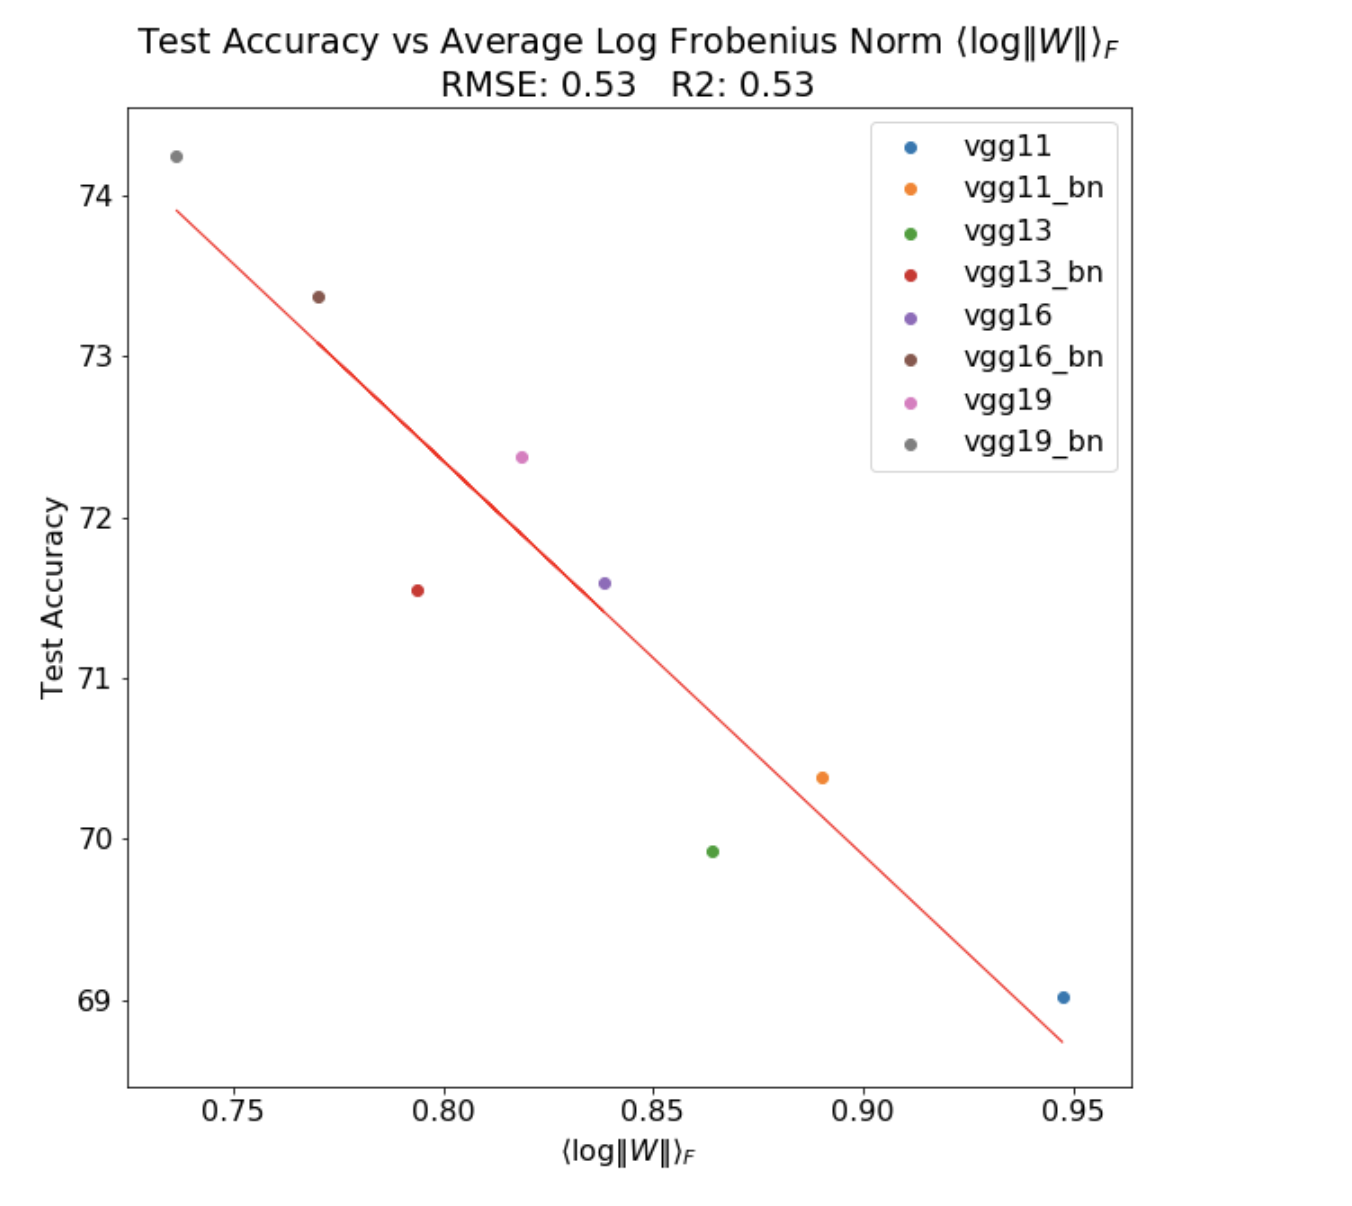
\includegraphics[width=5cm]{img/vgg-fnorm.png}
        \label{fig:vgg-fnorm}
    }
    \qquad
    \subfigure[ Spectral Norm ]{
        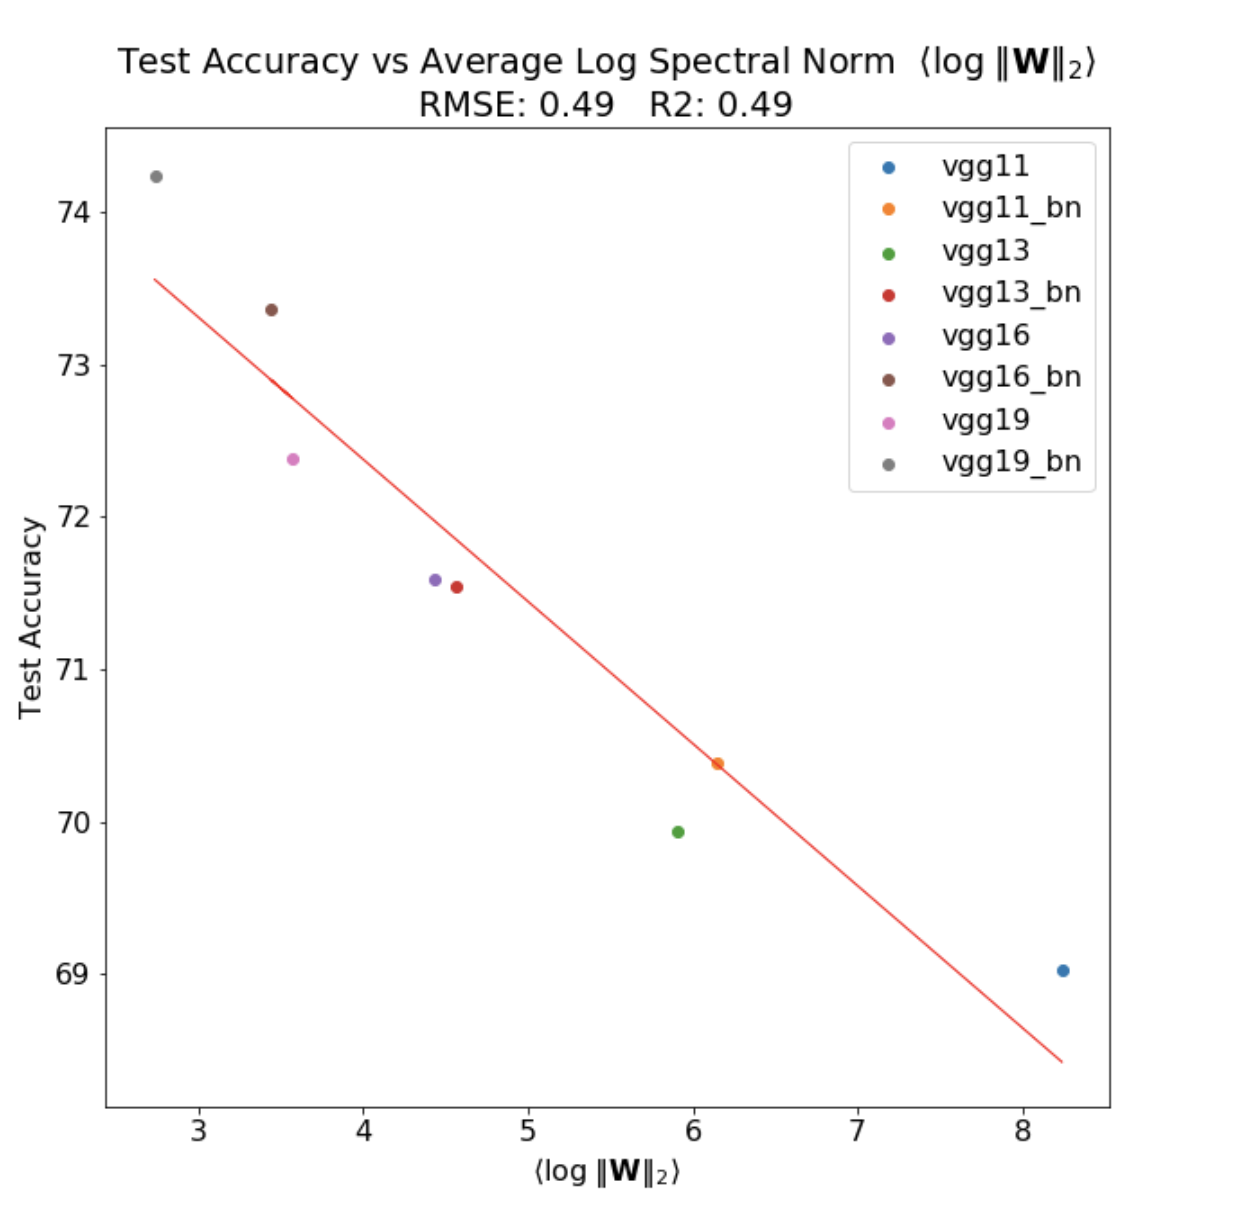
\includegraphics[width=4.9cm]{img/vgg-snorm.png}
        \label{fig:vgg-snorm}
    }
    \qquad
    \subfigure[ Weighted Alpha ]{
        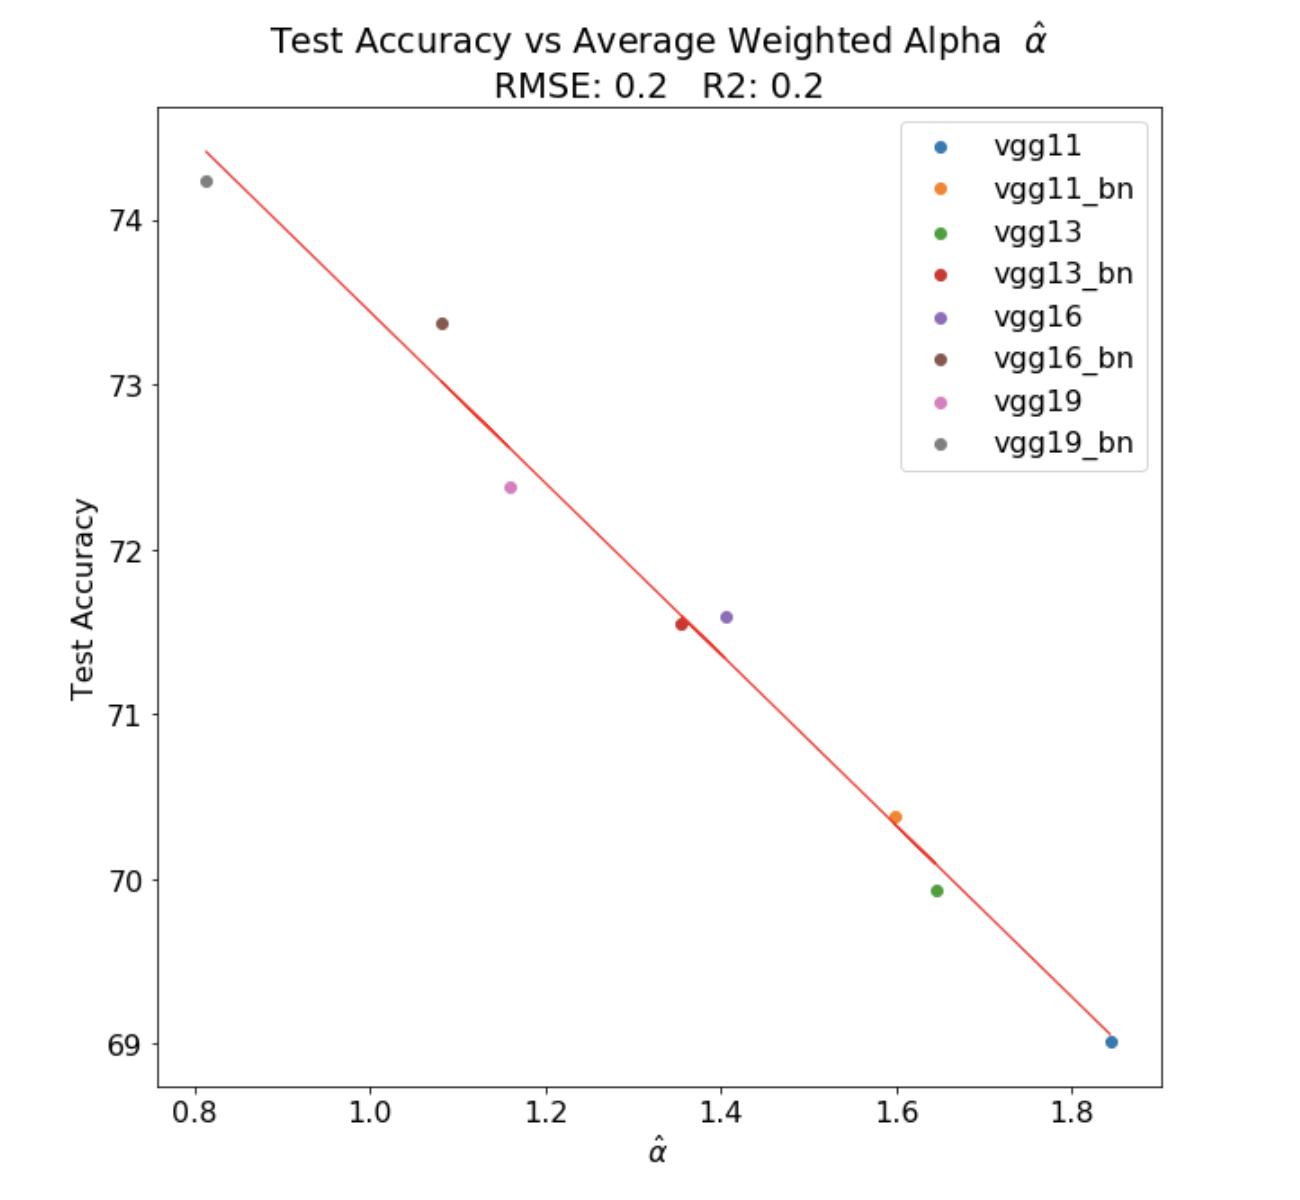
\includegraphics[width=4.9cm]{img/vgg-walpha.png}
        \label{fig:vgg-walpha}
    }
    \qquad
    \subfigure[ Alpha-Norm ]{
        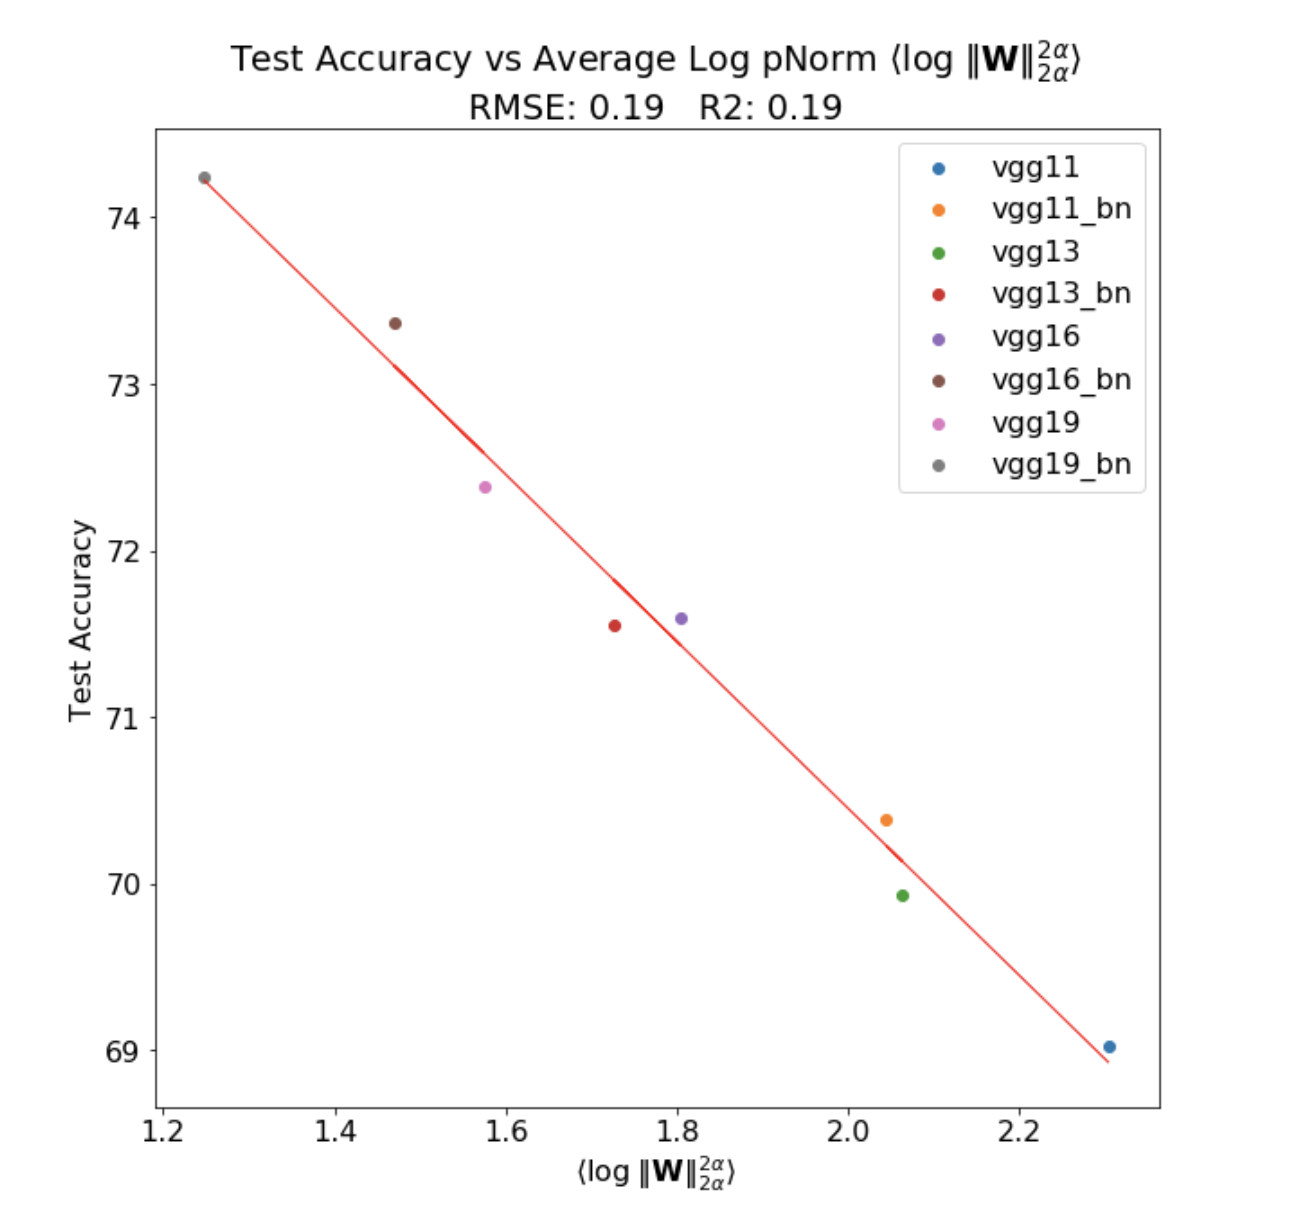
\includegraphics[width=4.9cm]{img/vgg-pnorm.png}
        \label{fig:vgg-pnorm}
    }
    \caption{Comparison of norm metrics vs reported test accuracy for pretrained VGG models, trained on ImageNet, available in pyTorch.  Plots will be updated and replace }
    

    \label{fig:vgg-metrics}
\end{figure}

ADD PLOTS FOR

pNorm and ResNet
pNorm and ResNet (ImageNet1K all models)
pNorm and DenseNet


\paragraph{Correlations and Information Flow in CV Models}

\begin{figure}[t]
    \centering

    \subfigure[ VGG ]{
        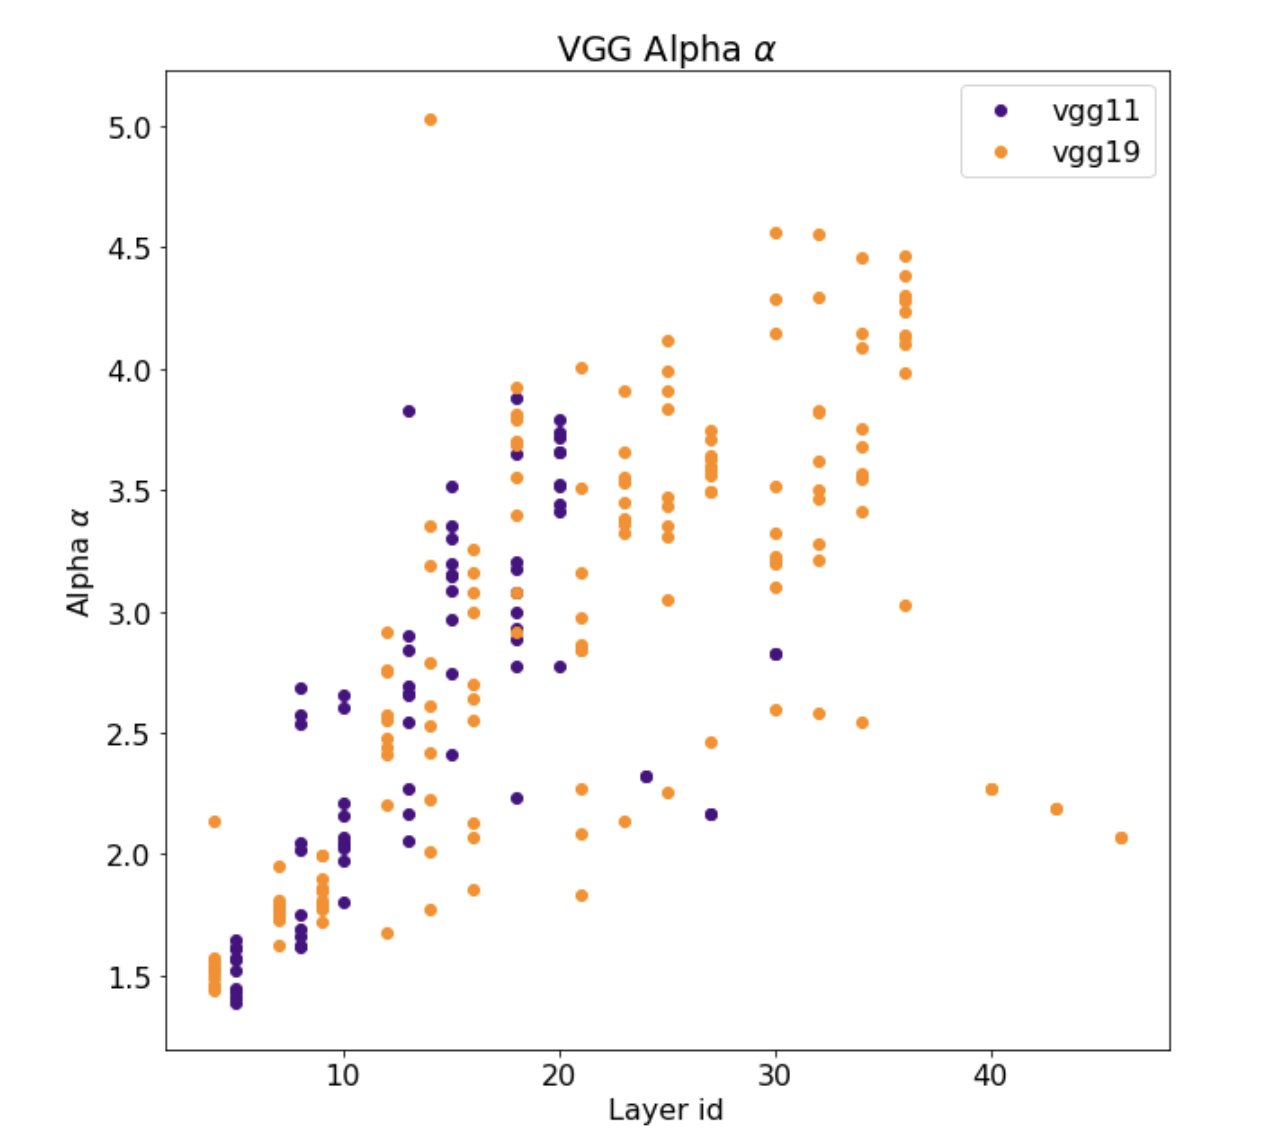
\includegraphics[width=4.1cm]{img/vgg-alpha-layers.png}
        \label{fig:vgg-alpha-layers}
    }
    \qquad
    \subfigure[ ResNet ]{
        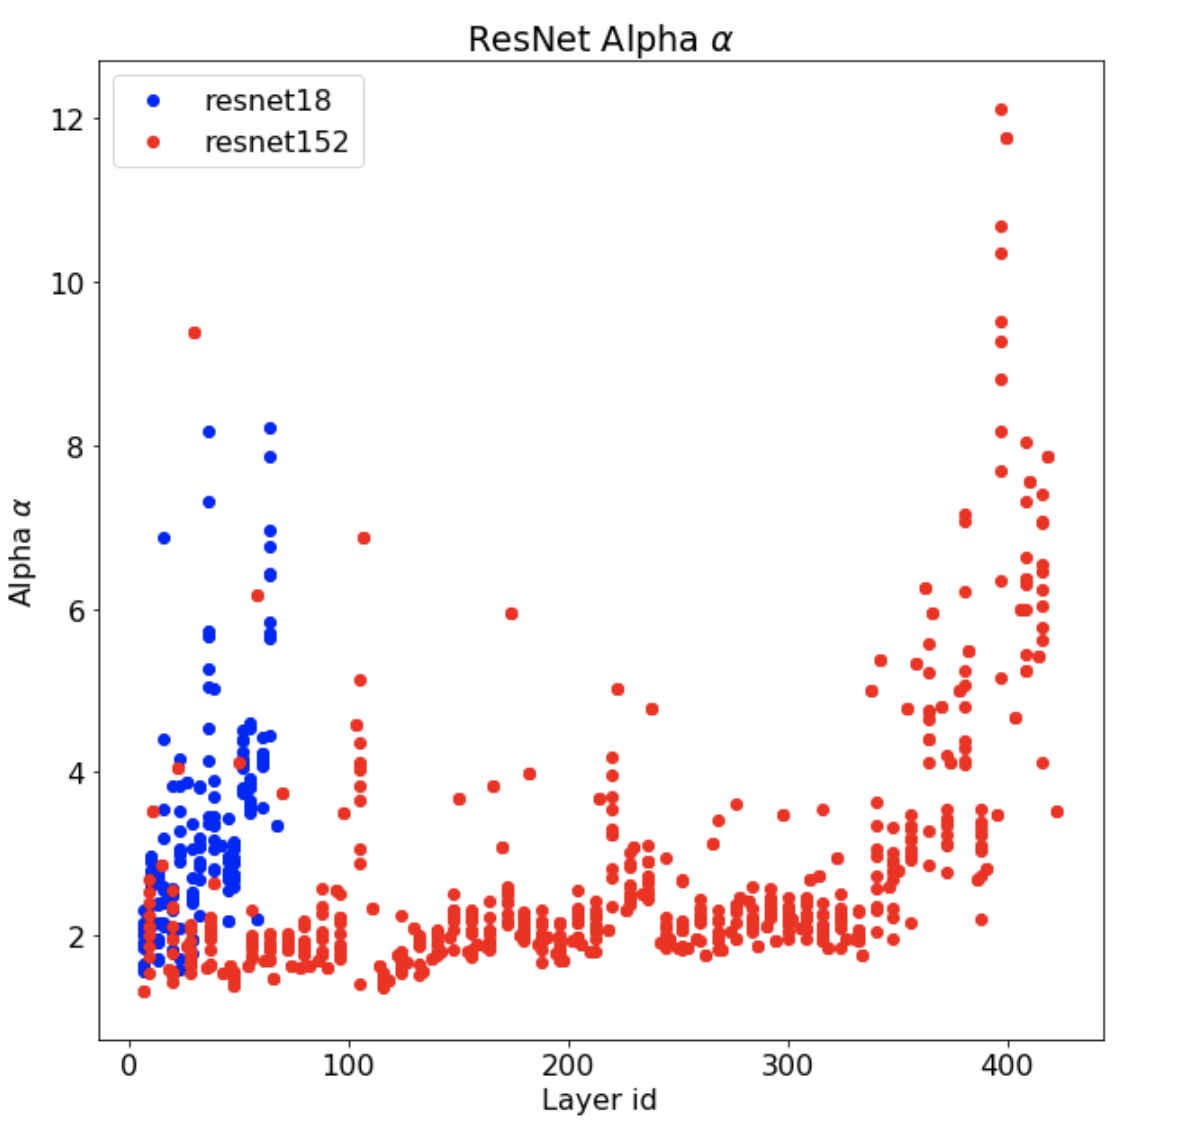
\includegraphics[width=3.8cm]{img/resnet-alpha-layers.png}
        \label{fig:resnet-alpha-layer}
    }
    \qquad
    \subfigure[ DenseNet ]{
        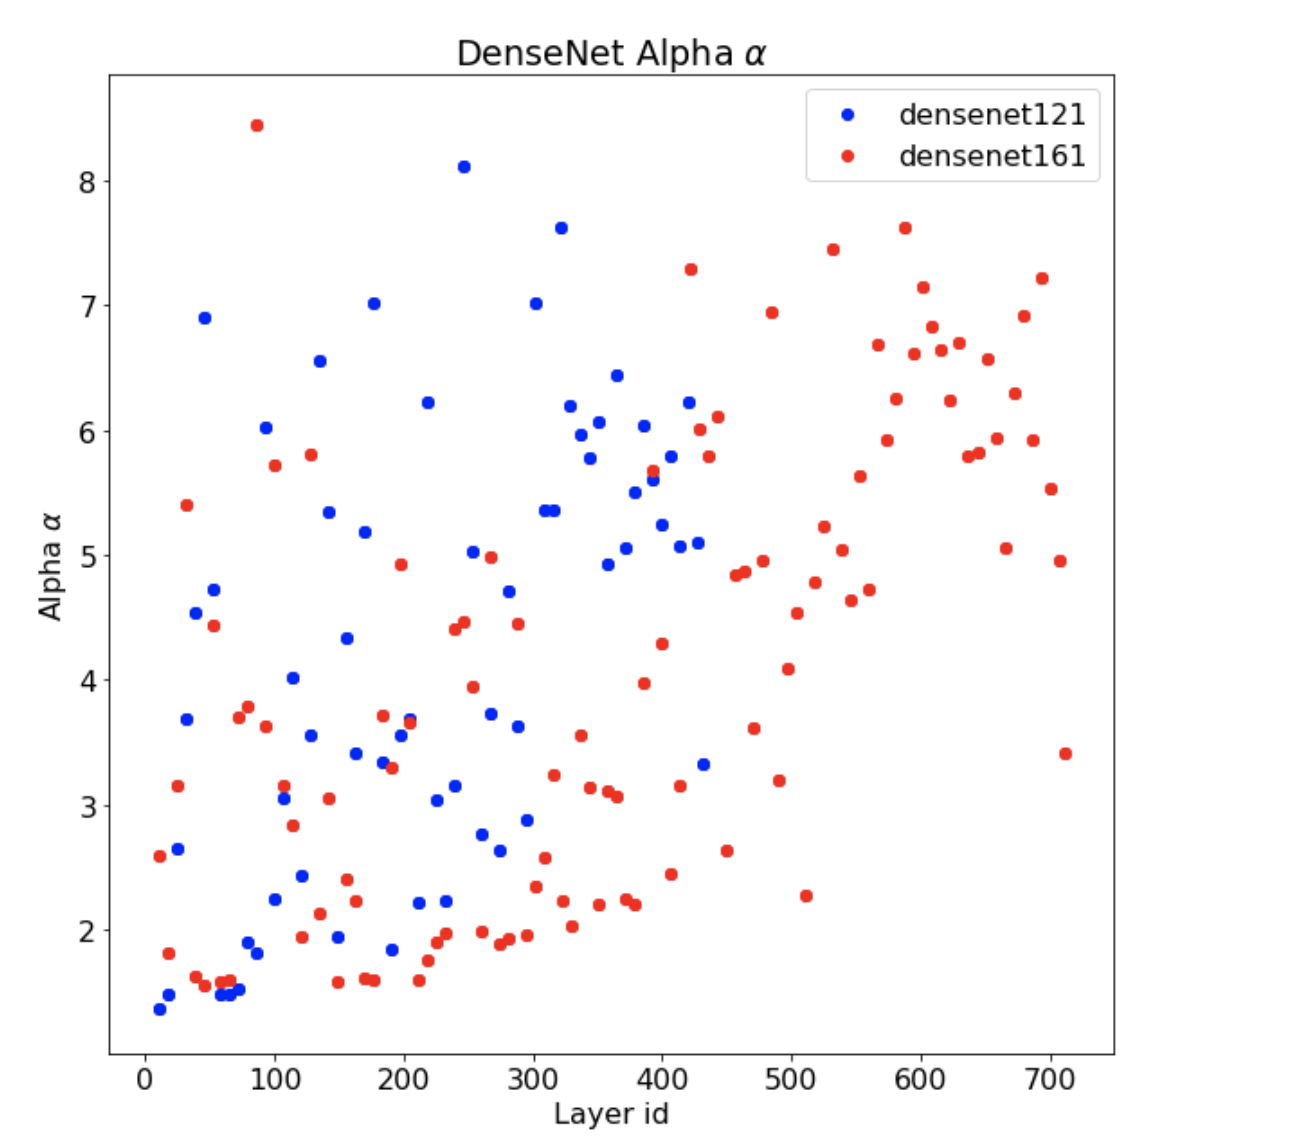
\includegraphics[width=4.1cm]{img/densenet-alpha-layers.png}
        \label{fig:densenet-alpha-layer}
    }
    \caption{Power law exponent $\alpha$ vs layer for VGG, ResNet, and DenseNet models}
    \label{fig:vgg-alpha-layers}
\end{figure}
